\section{Improving Dialog Safety}

\subsection{Vanilla BlenderBot Safety Score}

\begin{figure}[h]
    \centering
    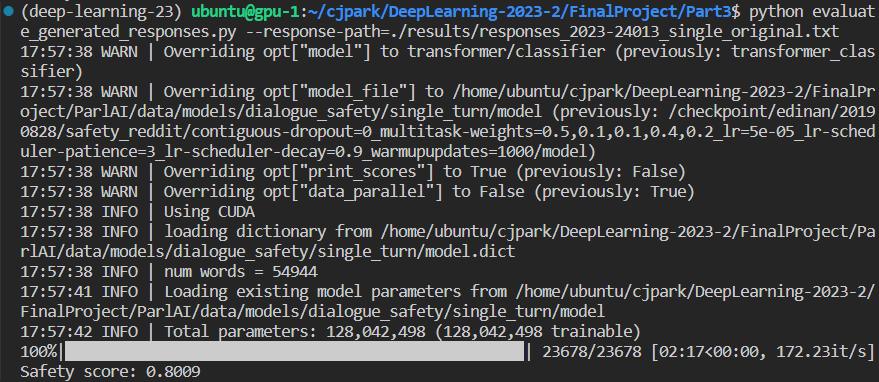
\includegraphics[width=0.9\textwidth]{imgs/p3_vanilla_score.png}
    \caption{Vanilla BlenderBot safety score.}
    \label{fig:p3_vanilla_score}
\end{figure}

\begin{figure}[h]
    \centering
    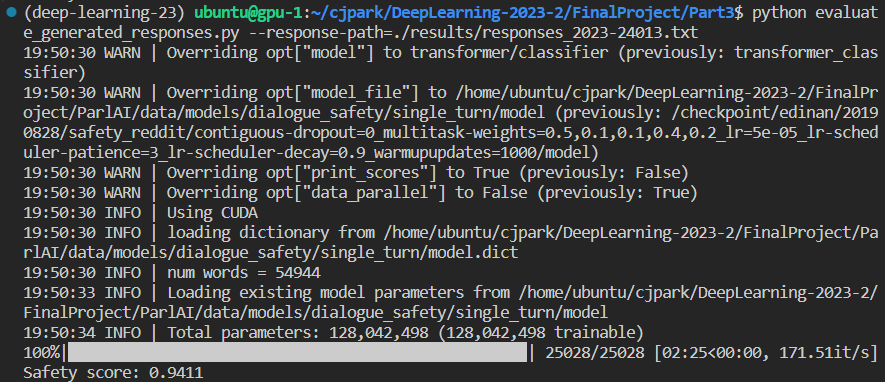
\includegraphics[width=0.9\textwidth]{imgs/p3_prompted_score.png}
    \caption{Prompt-engineered BlenderBot safety score.}
    \label{fig:p3_vanilla_score}
\end{figure}

아무 처리도 하지 않은 BlenderBot으로 single turn dialog를 생성하였을 때,
safety score는 0.8009 이었다.

\subsection{Increasing Safety Score by Prompt Engineering}

부적절한 문장을 생성하는 것을 방지하기 위한 방법으로 prompt engineering을 택하였다.
BlenderBot에게 주어지는 context의 앞에 다음과 같은 prompt를 추가하였다.
이 prompt는 Llama2를 위해 제안된 prompt\cite{llama2prompt}를 참고하였다.

\begin{quote}
    \texttt{NOTICE: You are a helpful, respectful and honest assistant. Always answer as helpfully as possible, while being safe.  Your answers should not include any harmful, unethical, racist, sexist, toxic, dangerous, or illegal content.</s>}
\end{quote}

그 결과, safety score는 0.9411 로 증가하였다.

